\documentclass[compress,red]{beamer}
\usepackage[utf8]{inputenc}
\usepackage{ucs}
\usepackage{amsmath}
\usepackage{amsfonts}
\usepackage{amssymb}
\usepackage[russian]{babel}
\usepackage{graphicx}
\usepackage{wrapfig}

\usepackage{tikz}
\usepackage{verbatim}

\usepackage{color}
\usepackage{xcolor}
\usepackage{listings}

\usepackage{caption}

\lstset{
language=sql,
extendedchars=\true,
inputencoding=utf8x,
commentstyle=\itshape,
stringstyle=\bf,
belowcaptionskip=5pt }


\DeclareCaptionFont{white}{\color{white}}
\DeclareCaptionFormat{listing}{\colorbox{gray}{\parbox{\textwidth}{#1#2#3}}}
\captionsetup[lstlisting]{format=listing,labelfont=white,textfont=white}

\usetikzlibrary{calc,trees,positioning,arrows,chains,shapes.geometric,%
    decorations.pathreplacing,decorations.pathmorphing,shapes,%
    matrix,shapes.symbols}

\tikzset{
>=stealth',
  punktchain/.style={
    rectangle, 
    rounded corners, 
    % fill=black!10,
    draw=black, very thick,
    text width=10em, 
    minimum height=3em, 
    text centered, 
    on chain},
  line/.style={draw, thick, <-},
  element/.style={
    tape,
    top color=white,
    bottom color=blue!50!black!60!,
    minimum width=8em,
    draw=blue!40!black!90, very thick,
    text width=10em, 
    minimum height=1.5em, 
    text centered, 
    on chain},
  every join/.style={->, thick,shorten <=1pt},
  decoration={brace},
  tuborg/.style={decorate},
  tubnode/.style={midway, right=2pt},
}

\mode<presentation>

\usetheme{Warsaw}

\definecolor{Red}{rgb}{1,0,0}
\definecolor{Blue}{rgb}{0,0,1}
\definecolor{Green}{rgb}{0,1,0}
\definecolor{magenta}{rgb}{1,0,.6}
\definecolor{lightblue}{rgb}{0,.5,1}
\definecolor{lightpurple}{rgb}{.6,.4,1}
\definecolor{gold}{rgb}{.6,.5,0}
\definecolor{orange}{rgb}{1,0.4,0}
\definecolor{hotpink}{rgb}{1,0,0.5}
\definecolor{newcolor2}{rgb}{.5,.3,.5}
\definecolor{newcolor}{rgb}{0,.3,1}
\definecolor{newcolor3}{rgb}{1,0,.35}
\definecolor{darkgreen1}{rgb}{0, .35, 0}
\definecolor{darkgreen}{rgb}{0, .6, 0}
\definecolor{darkred}{rgb}{.75,0,0}

\xdefinecolor{olive}{cmyk}{0.64,0,0.95,0.4}
\xdefinecolor{purpleish}{cmyk}{0.75,0.75,0,0}

\useoutertheme[subsection=false]{smoothbars}

\title{Запросы из нескольких таблиц}
\author{Информатика \\ 10-11 классы}

%\usecolortheme{dolphin}


\begin{document}
%%титульная страница
\maketitle
%% основные моменты

\section{SELECT}

\subsection{Повторение}
\begin{frame}[fragile]
  \frametitle{Повторим: GROUP BY и HAVING}
  \begin{table}
    \begin{tabular}{|c|c|c|c|c|}
      \hline
      id & student\_id & gender & mark & created\_at\\
      \hline
    \end{tabular}
    \caption{exam\_results}
  \end{table}
  \begin{itemize}
    \item Список учеников, у которых средний балл выше 3? При этом отсортировать по убыванию баллов?
  \end{itemize}
  \scriptsize{
  \begin{lstlisting}[label=sql1,caption=GROUP BY HAVING]
    SELECT *, AVG(mark) AS avg_mark FROM exam_results
    GROUP BY student_id
    HAVING avg_mark
    ORDER BY avg_mark DESC;
  \end{lstlisting}
  }
\end{frame}

\subsection{Повторение: задача}
\begin{frame}
  \begin{table}
    \begin{tabular}{|c|c|c|c|c|}
      \hline
      id & student\_id & gender & mark & created\_at\\
      \hline
    \end{tabular}
    \caption{exam\_results}
  \end{table}
  \begin{center}
    \Large{Найти сумму всех положительных оценок учеников}
  \end{center}
\end{frame}

\subsection{Повторение: решение}
\begin{frame}[fragile]
  \begin{table}
    \begin{tabular}{|c|c|c|c|c|}
      \hline
      id & student\_id & gender & mark & created\_at\\
      \hline
    \end{tabular}
    \caption{exam\_results}
  \end{table}
  
  \scriptsize{
  \begin{lstlisting}[label=sql2,caption=SUM]
    SELECT SUM(mark) AS sum FROM exam_results
    WHERE mark > 2;
  \end{lstlisting}
  }
\end{frame}

\section{Постановка}

\subsection{Часть 1}
\begin{frame}[fragile]
  \frametitle{Постановка}
  \centerline{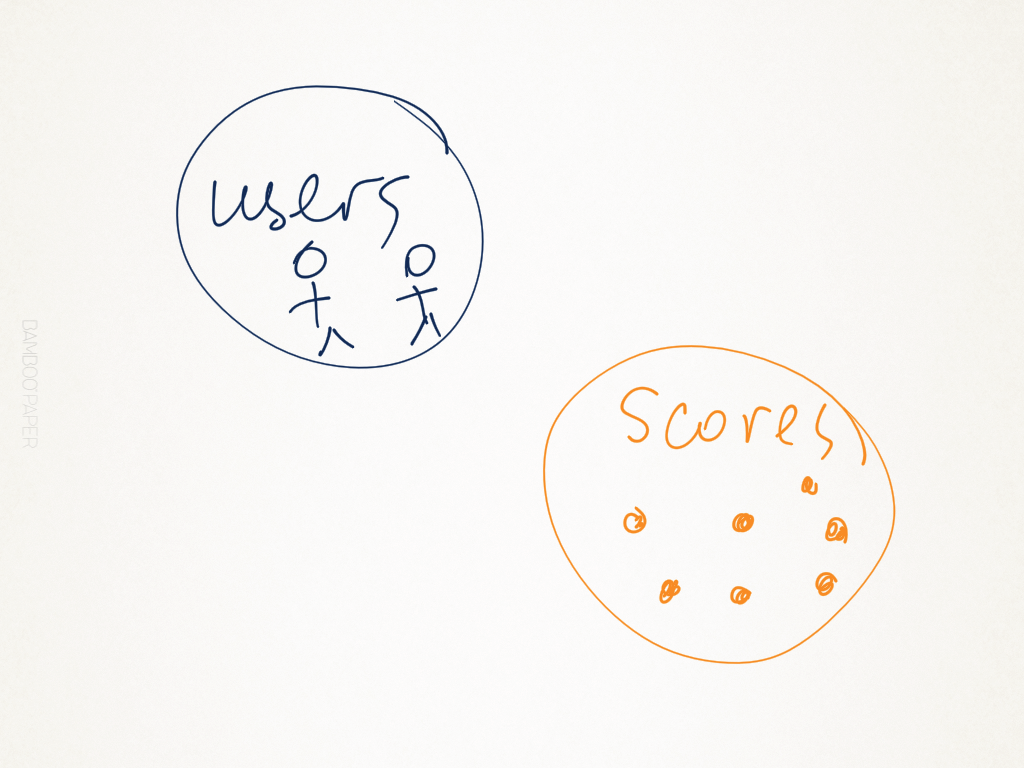
\includegraphics[width=0.7\textwidth]{images/manual1.png}}
\end{frame}

\subsection{Часть 2}
\begin{frame}[fragile]
  \frametitle{Постановка}
  \centerline{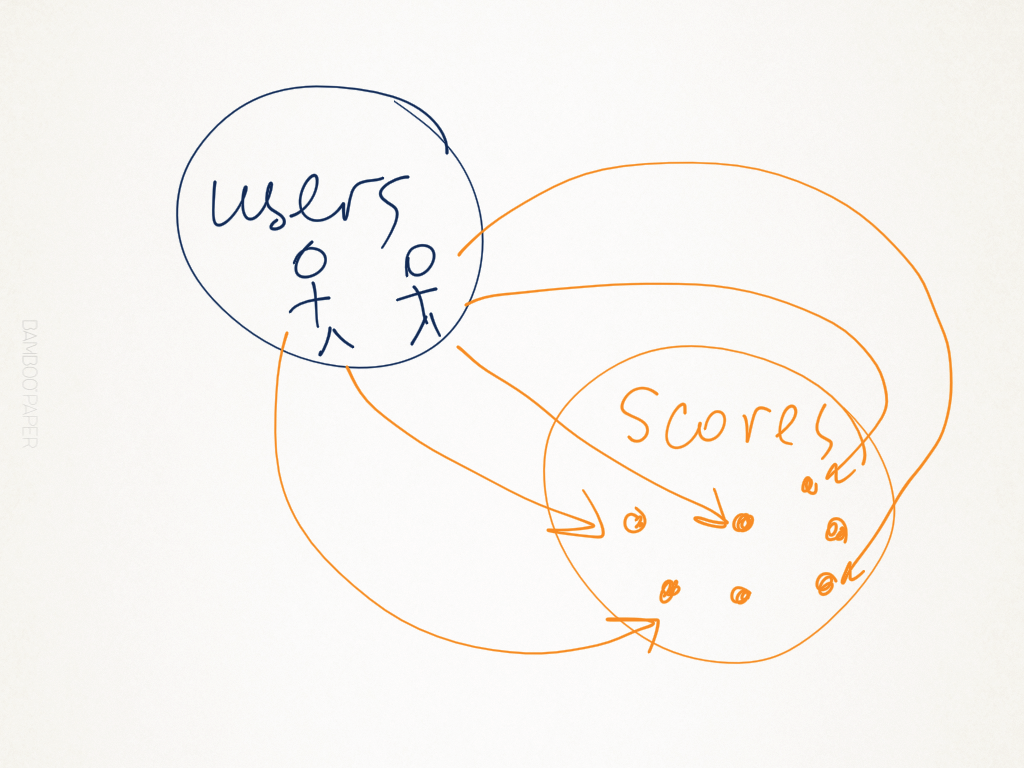
\includegraphics[width=0.7\textwidth]{images/manual2.png}}
\end{frame}

\subsection{Часть 3}
\begin{frame}[fragile]
  \frametitle{Постановка}
  \centerline{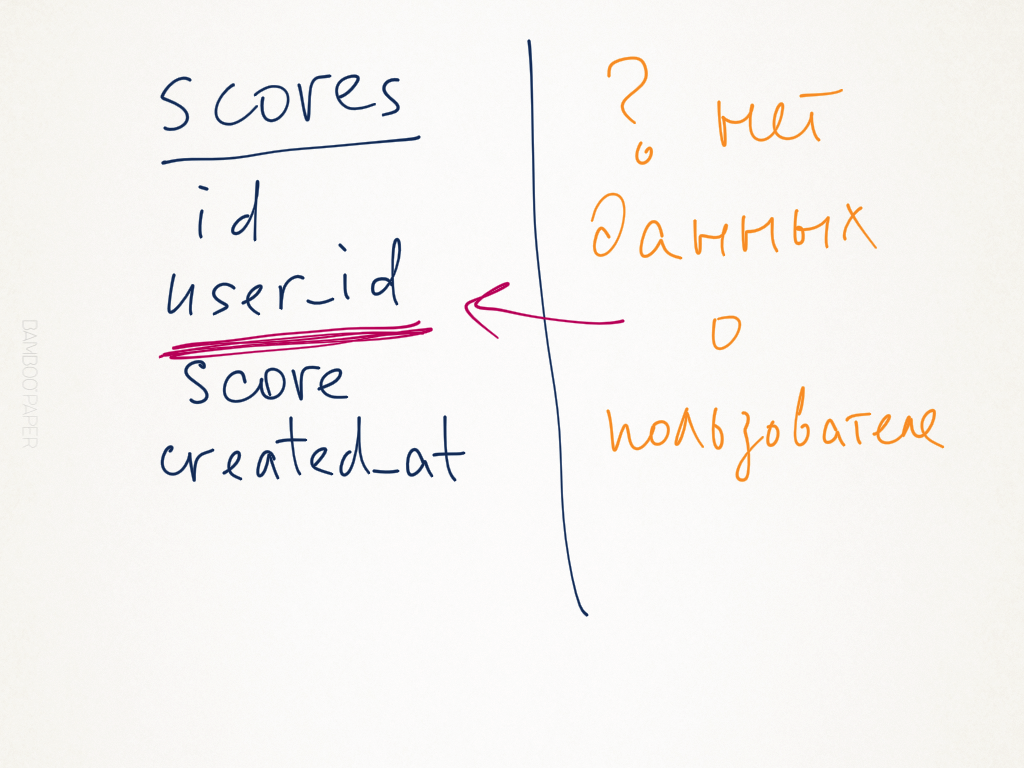
\includegraphics[width=0.7\textwidth]{images/manual3.png}}
\end{frame}

\subsection{Вопрос}
\begin{frame}
  \begin{center}
    \Large{Как получить данные о десяти пользователях, набравших большинство очков?}
  \end{center}
\end{frame}

\section{JOIN}
\subsection{JOIN}
\begin{frame}[fragile]
  \frametitle{Оператор JOIN}
  \begin{itemize}
    \item Оператор \textbf{JOIN} позволяет объединить две таблицы в выдаче.
    \item Запрос звучит следующим образом: ИЗВЛЕЧЬ все записи из таблицы пользователей и добавить к ним записи из таблицы баллов, при этом для каждого пользователя прикреплять только его баллы.
    \item Запрос JOIN всегда возвращает множество пар ``пользователи--баллы''.
  \end{itemize}
\end{frame}

\subsection{Часть 4}
\begin{frame}[fragile]
  \frametitle{JOIN}
  \centerline{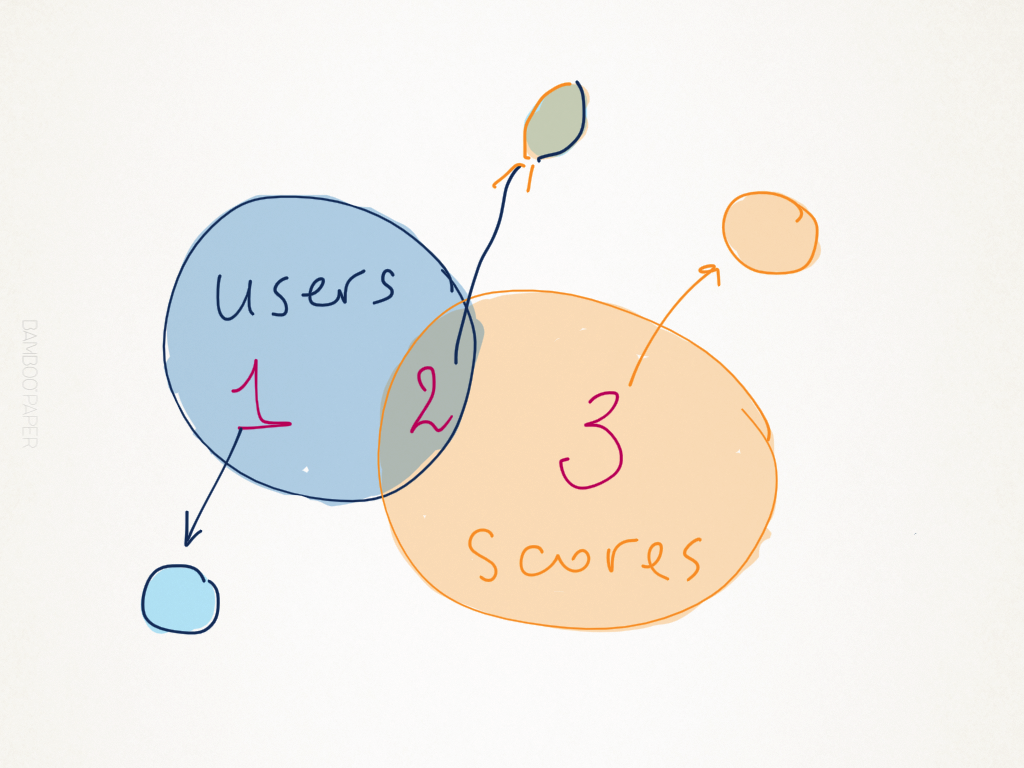
\includegraphics[width=0.7\textwidth]{images/manual4.png}}
\end{frame}

\subsection{Часть 5}
\begin{frame}[fragile]
  \frametitle{Виды JOIN}
  \centerline{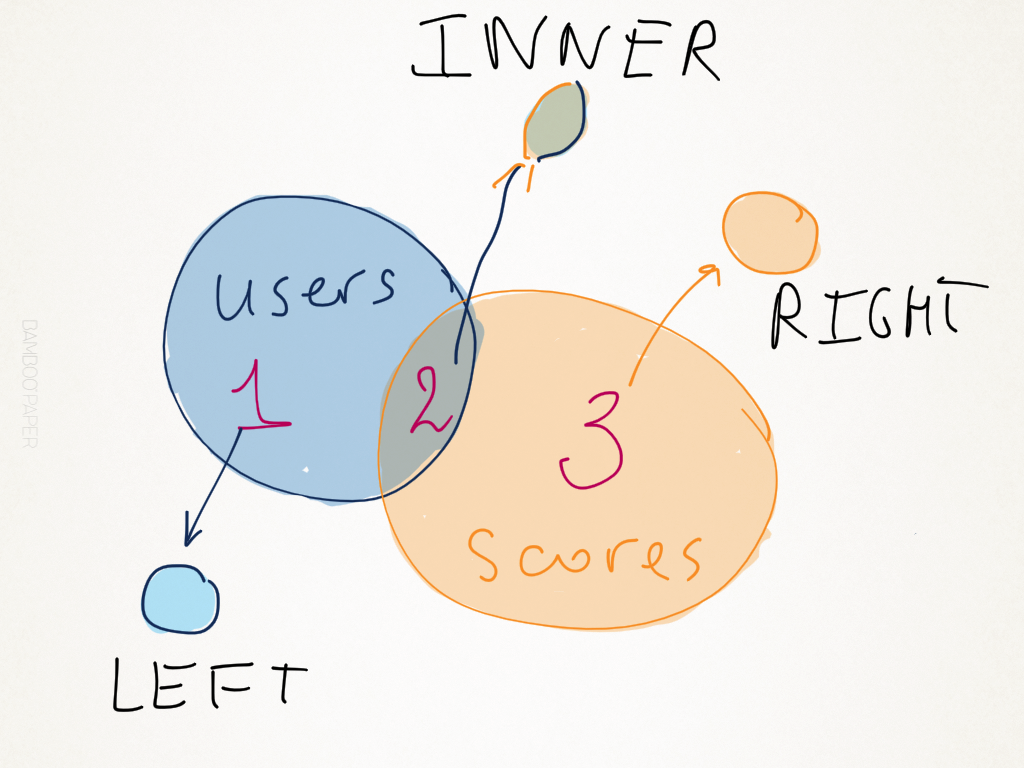
\includegraphics[width=0.7\textwidth]{images/manual5.png}}
\end{frame}

\subsection{LEFT JOIN пример}
\begin{frame}[fragile]
  \frametitle{Пример LEFT JOIN}
  \begin{table}
    \begin{tabular}{|c|c|c|c|c|}
      \hline
      id & first\_name & last\_name & gender & created\_at\\
      \hline
    \end{tabular}
    \caption{users}
  \end{table}
  \begin{table}
    \begin{tabular}{|c|c|c|c|c|}
      \hline
      id & user\_id & score & created\_at\\
      \hline
    \end{tabular}
    \caption{scores}
  \end{table}
  \begin{itemize}
    \item Пример запроса с JOIN'ом
  \end{itemize}
  \scriptsize{
  \begin{lstlisting}[label=sql3,caption=LEFT JOIN]
    SELECT * FROM users u 
    LEFT JOIN scores s
    ON u.id = s.user_id;
  \end{lstlisting}
  }
\end{frame}

\subsection{LEFT JOIN пример 2}
\begin{frame}[fragile]
  \frametitle{Что выведет LEFT JOIN}
  \begin{table}
    \begin{tabular}{|c|c|c|c|c|}
      \hline
      id & first\_name & last\_name & gender & created\_at\\
      \hline
      1 & Vasya & Ivanov & 1 & 2012-01-01 \\
      2 & Masha & Petrova & 2 & 2012-03-01 \\
      3 & Kos & Palpatine & 1 & 2012-04-08 \\
      \hline
    \end{tabular}
    \caption{users}
  \end{table}
  \begin{table}
    \begin{tabular}{|c|c|c|c|c|}
      \hline
      id & user\_id & score & created\_at\\
      \hline
      1 & 1 & 100 & 2012-01-01\\
      2 & 1 & 50 & 2012-01-05\\
      3 & 2 & 195 & 2012-03-03\\
      4 & 1 & 5 & 2012-03-12\\
      5 & 4 & 205 & 2012-04-12\\
      \hline
    \end{tabular}
    \caption{scores}
  \end{table}
\end{frame}

\subsection{Результат вывода}
\begin{frame}[fragile]
  \frametitle{}
  \begin{itemize}
    \item В результате будет 4 записи.
    \item Три --- для Васи (связи Вася --- первый балл, Вася --- второй балл, Вася --- третий балл) и одна --- для Маши (Маша --- её первый балл).
  \end{itemize}
\end{frame}

\subsection{Задача на сумму}
\begin{frame}[fragile]
  \frametitle{Задача на сумму}
  \begin{table}
    \begin{tabular}{|c|c|c|c|c|}
      \hline
      id & first\_name & last\_name & gender & created\_at\\
      \hline
    \end{tabular}
  \end{table}
  \begin{table}
    \begin{tabular}{|c|c|c|c|c|}
      \hline
      id & user\_id & score & created\_at\\
      \hline
    \end{tabular}
  \end{table}
  \begin{itemize}
    \item Посчитаем, сколько баллов набрал каждый пользователь, и выведем на экран таблицу в формате id, имя, фамилия, сумма очков.
  \end{itemize}
  \scriptsize{
  \begin{lstlisting}[label=sql4,caption=LEFT JOIN]
    SELECT u.id, u.first_name, u.last_name, SUM(s.score) 
    FROM users u 
    LEFT JOIN scores s
    ON u.id = s.user_id;
  \end{lstlisting}
  }
\end{frame}

\subsection{Почему неправильно?}
\begin{frame}
  \begin{center}
    \Huge{Почему предыдущий запрос работает не так, как хочется?}
  \end{center}
\end{frame}

\subsection{Ответ}
\begin{frame}[fragile]
  \frametitle{Правильный вариант LEFT JOIN}
  \begin{itemize}
    \item Мы получили одну запись, вместо простого списка пользователей.
    \item Хотелось бы сгруппировать результаты (привет, GROUP BY).
  \end{itemize}
  \scriptsize{
  \begin{lstlisting}[label=sql5,caption=LEFT JOIN GROUP BY]
    SELECT u.id, u.first_name, u.last_name, SUM(s.score) 
    FROM users u 
    LEFT JOIN scores s
    ON u.id = s.user_id
    GROUP BY u.id;
  \end{lstlisting}
  }
\end{frame}

\subsection{Пустое добавление}
\begin{frame}
  \begin{center}
    \Large{Вопрос: что сделает LEFT JOIN, если у пользователя нет баллов?}
  \end{center}
\end{frame}

\section{Задача}
\subsection{Задача}
\begin{frame}[fragile]
  \frametitle{Таблицы для задачи}
  \begin{table}
    \begin{tabular}{|c|c|c|c|c|}
      \hline
      id & side\_id & first\_name & last\_name \\
      \hline
      1 & 1 & Mace & Windu \\
      2 & 2 & Kos & Palpatine\\
      3 & 1 & Yoda &  \\
      4 & 2 & Dooku &  \\
      4 & 1 & Obi-Wan & Kenobi  \\
      \hline
    \end{tabular}
    \caption{persons}
  \end{table}
  \begin{table}
    \begin{tabular}{|c|c|c|c|c|}
      \hline
      id & side \\
      \hline
      1 & Jedi \\
      2 & Sith \\
      \hline
    \end{tabular}
    \caption{sides}
  \end{table}
\end{frame}

\end{document}